\subsection{Phase Diagram}
In order to visualize the different regimes of Cooper pairing, a phase diagram for the superconductor is constructed.
It provides information about which pairing state is favored for which combination of parameters.
In our case, the dependency on the RKKY-interaction strength is of special interest.
For a conclusive interpretation of a phase diagram which shows the dependency on the RKKY-interaction strength, it is necessary to understand the unperturbed system first.
That allows to choose the parameters such that the initial state for zero RKKY-interaction strength is known. \newline
The phase of the system is determined by comparing the amplitudes of the different spin pairings for several parameter sets. 
These amplitudes are specified in Eq. \ref{eq:spin-pairing-amplitudes} and their comparison yields the phase diagrams presented in the next sections.

\subsubsection{SOC dependent}
The free-energy determined in Sec. \ref{sec:free_energy} is calculated numerically for different sets of parameters, leading to the phase diagram in Figure \ref{fig:phasediagramm_unperturbed}.
It is visible that.... INTERPRETATION 

\begin{figure}[h]
    \centering
    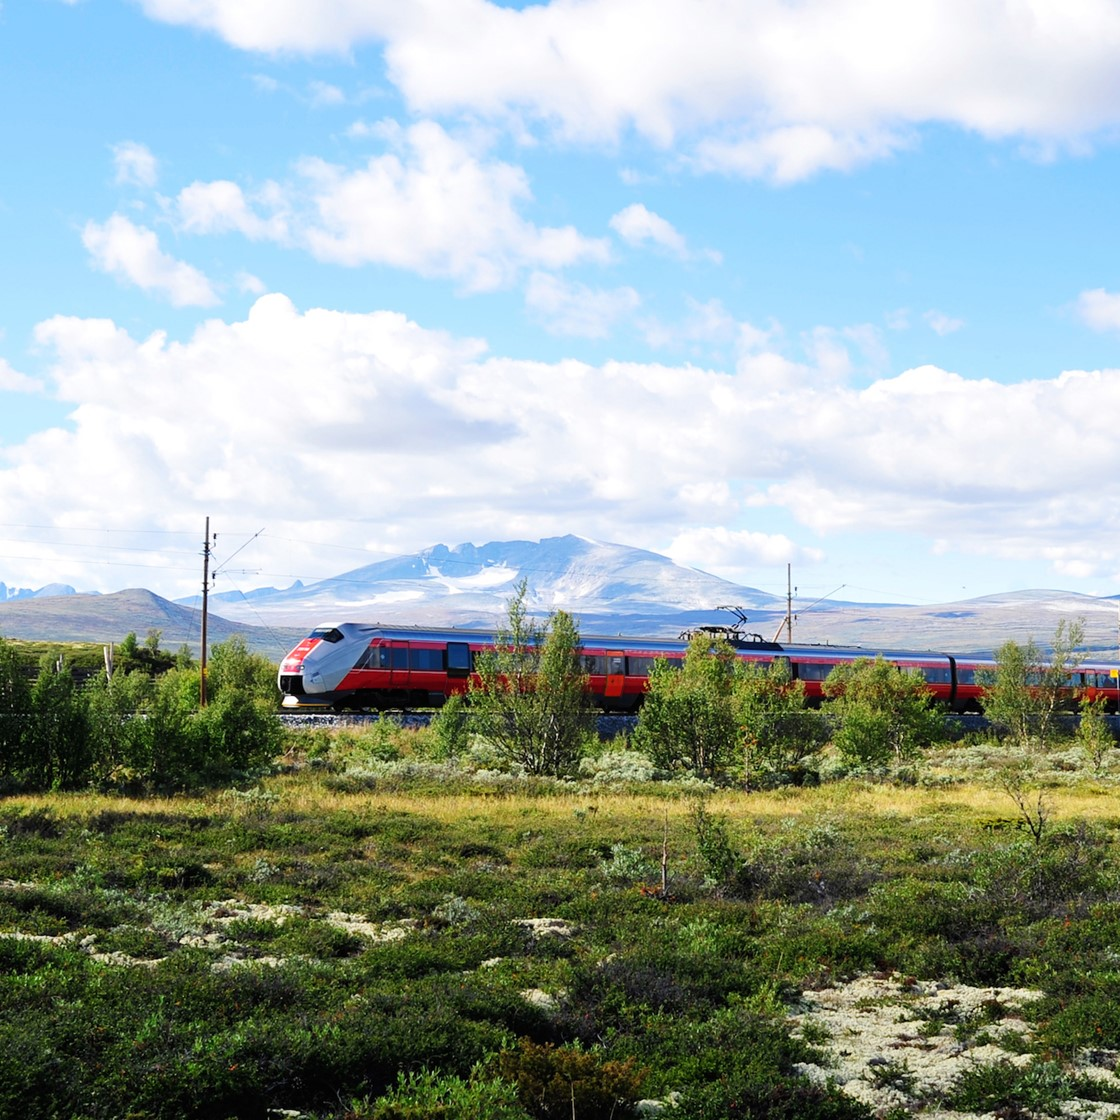
\includegraphics[width=0.5\textwidth]{Images/beispiel.png}
    \caption{Phase diagram of unperturbed system.}
    \label{fig:phasediagramm_unperturbed}
\end{figure}